\documentclass{sig-alternate}
\usepackage{graphicx}
\usepackage{amsmath}
\usepackage{amssymb}
\usepackage{natbib}
\usepackage{myAlgorithm}
\usepackage{xcolor}

\bibliographystyle{abbrvnat}

\definecolor{darkred}{rgb}{.5,0,0}


%XXX:  Machine Learning for Auto-tuning: A Data-Drive Approach...} ???
%\title{Boosted Regression Trees for Data-Driven Auto-Tuning}
\title{Boosted Regression Trees for Predictive Auto-Tuning}
% NP: I like this title !
%XXX:  Machine Learning for Auto-tuning: A Data-Drive Approach...} ???

\numberofauthors{3}

\author{
%\alignauthor First Last\titlenote{}\\
\alignauthor First Last\\
\affaddr{Affiliation line 1}\\
\affaddr{Affiliation line 2}\\
\email{anon@mail.com}
% 2nd author
%\alignauthor First Last\titlenote{None}\\
\alignauthor First Last\\
\affaddr{Affiliation line 1}\\
\affaddr{Affiliation line 2}\\
\email{anon@mail.com}
% 3rd author
%\alignauthor First Last\titlenote{None}\\
\alignauthor First Last\\
\affaddr{Affiliation line 1}\\
\affaddr{Affiliation line 2}\\
\email{anon@mail.com}
}

\begin{document}
\maketitle

\begin{abstract}
Template-based auto-tuning techniques are widely used and effective for optimizing a
parametrized GPU code template for a particular computation on particular
hardware \cite{XXXX}.  A drawback of this approach is that exhaustive, or even thorough, auto-tuning requires
compiling many kernels and calling each one many times, and this process is slow.
Furthermore, library abstraction boundaries provide operations such as image
filtering and matrix multiplication, which actually correspond to a large set
of potential problem configurations with a wide variety of memory access
patterns and computational bottlenecks.  How can we draw on data from previous
empirical auto-tuning of related problems on related hardware to make a
just-in-time implementation decision for a novel problem?  This paper presents
a machine learning approach to auto-tuning, in which features of the
current hardware platform, the kernel configuration and the problem
instance are passed to a regression model (boosted regression trees) which
predicts how much faster this kernel will be than a reference baseline.
Combinatorial optimization strategies that would normally implement auto-tuning
by evaluating kernel configurations on the real hardware are orders of
magnitude faster when evaluating the surrogate regression model instead.  We
validate our approach using the filterbank correlation kernel described in
\citet{pinto+cox:2011gcg}, where we find that 0.1 seconds (XXX) of hill
climbing on the regression model ({\em predictive} auto-tuning) can achieve an
average of 95\% of the speed brought by 120 seconds of empirical auto-tuning
XXX.  Our approach is not specific to filterbank correlation, nor to GPU
kernel auto-tuning; the approach of using a non-linear regression model on top
of simple features applies to a variety of problem types, kernel types, and
platforms.  \end{abstract}

\section{Introduction}

% 1 Introduction

% HPC Landscape: from single proc to multi-cores

Due to power consumption and heat dissipation concerns, scientific applications
have shifted from computing platforms where performance had been primarily
driven by rises in the clock frequency of a single ``heavy-weight'' processor
(with complex out-of-order control and cache structures) to a platform with
ever increasing numbers of ``light-weight'' cores. Interestingly, this shift is
now not only relevant to computational sciences but to the development of all
computer systems: from ubiquitous consumer-facing devices (e.g. phones) to
high-end computer farms for web-scale applications (e.g. social networks).

% HPC Landscape: large diversity of architectures,
% no consensus => push to flexibility => push to sw

Although the future lies in low-power multi-core hardware designs, the field
lacks  consensus on exactly how the different subsystems (memory,
communication and computation) should be efficiently integrated, modeled and
programmed. These systems have exhibited varying degrees of memory hierarchy
and multi-threading complexity and, as a consequence, they have been
increasingly relying on flexible but low-level software-controlled cache
management and parallelism \citep{asanovic2006landscape} in order to better
control and understand the various trade-offs among performance, reliability,
energy efficiency, production costs, etc. This evolution has profoundly
altered the landscape of application development: programmers are now
facing a wide diversity of low-level architectural features to write
high-performance \emph{and} portable code.

\subsection{Motivation}

% Better tools: motivation (compilers/tools/libs can’t keep up, it’s too
% difficult)

In this rapidly evolving landscape, the construction of \emph{general}
development tools and libraries that \emph{fully utilize} system resources
remains a daunting task. Even within specialized architectures from the
\emph{same} vendor, like NVIDIA's Graphics Processing Units (GPUs) and the
Compute Unified Device Architecture (CUDA) \citep{nickolls2008scalable,
nvidia2011cuda}, many developers default to massive amounts of manual labor
to optimize CUDA code to specific input domains. In addition, hand-tuning
rarely generalizes well to new hardware generations or different input
domains, and it can also be error-prone or far from optimal. One of the
reason is that kernels can produce staggeringly large optimization spaces
\citep{datta2008stencil}. The problem is further compounded by the fact that
these spaces can be highly discontinuous \citep{ryoo2008program}, difficult
to explore and holding quasi-optimal solutions at the edge of ``performance
cliffs'' (in part due to hard resource restrictions, like the register file
size).

\subsection{Auto-Tuning}
% Related Work instead ??

% auto-tuning is an answer

One strategy for addressing these challenges is to use one of a variety of automatic
methods known collectively as ``auto-tuning''. Two major auto-tuning approaches have emerged
in the extensive literature covering the subject (see surveys in
\citep{vuduc2001statistical, demmel2005self, vuduc2005oski, williams2008auto,
datta2008stencil, cavazos2008intelligent, li2009note, park2011evaluation}):
analytical model-driven optimization and empirical optimization
\citep{yotov2003comparison}.

% model-driven optimization: intro

The model-driven optimization approach uses analytical abstractions to model
the hardware architectures, the possible code transformations and their complex
interactions. Even though highly-accurate analytical models are generally
intractable to build, this approach has been quite successful in the past at
accelerating serial code with simplified but general abstractions. However,
large speed-ups for parallel code require more accurate high-dimensional models
and since this approach is bound by the quality and scalability of its
abstraction, it has been less suited for highly-specialized kernels. This
approach has been dominant in the compiler community. As a result, it has
generally been applied at compile-time where important run-time characteristics
such as input domains are missing. These drawbacks render the model-driven
optimization approach less attractive for high-performance library developers.

% * empirical optimization: intro / advantages

The empirical optimization approach, on the contrary, seeks to find the best
performing code configuration by automatically generating many versions of a
parametrized kernel and benchmarking them on the actual hardware (possibly at
runtime, when contextual information about the hardware and software stack is
the richest). This method directly optimizes the metric(s) of interest and not
surrogates. One of its main advantage is that it allows any metric to be
optimized without loss of generality. It is indeed possible to formulate the
problem as a multi-objective optimization and minimize both speed \emph{and}
power consumption \citep{rahman2011automated}, a feat that renders the
analytical model-driven approach even more difficult. Due to its flexibility,
empirical auto-tuning has been successfully applied to build high-performance
domain-specific libraries including dense linear algebra
\citep{clint2001automated, bilmes1997optimizing}, sparse linear algebra
\citep{vuduc2005oski}, signal processing \citep{frigo1998fftw}, sorting
\citep{li2004dynamically}, general stencil operations \citep{kamil2010auto}, etc.

Even though such a ``black-box'' approach does not try to build an
explicit model per se, it could, if care were taken, help to greatly accelerate
our understanding of the complex interactions between the set of optimizations,
their parameters and the hardware architectural features (XXX: that's what
we are trying to do w/ ML-based, decision trees, etc.).

% empirical optimization: disadvantages

The empirical approach is very sensitive to the choice of instrumented
optimizations \emph{and} to the search method. The size of the search space is
so large that the current best empirical auto-tuners can only consider
highly-specialized functions with a limited set of code transformations and
compiler options, on very few input domains \citep{ganapathi2009case}. Although
searching for good code configurations in this highly-discontinuous space can
be made embarrassingly parallel, it remains a very difficult and prohibitively
expensive combinatorial optimization problem as many variants of the code must
generated, compiled, and benchmarked on specific input domains with meaningful
statistics (that may require multiple runs). Consequently, most proposed
methods prune the space with hard-coded heuristics that offer little
generalization guarantees. This has been the main drawback of the empirical
approach compared to the model-driven approach where good code configurations
can be directly derived from the analytical model.

% hybrid optimization: the bad way

To alleviate this major weakness, it is intuitively appealing to combine the two
approaches by first constraining the search space with an analytical model and
then exploring the reduced space empirically \citep{chen2005combining,
li2009note}. Unfortunately, this hybrid approach is still bound by the quality
of the analytical model, which remains hard to build by hand.

% hybrid optimization: the ML way (note that ML-based are in essence
% model-driven too just with an empirically learned model)

In this paper, we propose to \emph{learn the model}, empirically, (XXX:
we'll describe what this means in more details later in the paper, riiiighhht
???) instead of deriving it analytically. By learning the model, one can
hope to achieve elements of the best of both approaches and capitalize on the large body of
literature from the machine learning community.

Although various statistical prediction techniques have been applied with
success at compile-time for general programs on various CPU architectures
\citep{monsifrot2002machine, stephenson2003meta, yotov2003comparison,
kulkarni2004fast, cooper2005acme, franke2005probabilistic,
hutter2006performance, cavazos2007rapidly, cavazos2008intelligent,
hartono2009annotation, park2011evaluation, fursin2008milepost}, there is, to
our knowledge, no fast predictive auto-tuning work that has tried to cover
simultaneously: (a) more recent multi-core architectures like GPUs
\citep{schaa2009exploring}, (b) high-performance domain-specific libraries
\citep{nukada2009auto, li2009note, kamil2010auto}, (c) at run-time
\citep{klockner2011pycuda, pinto+cox:2011gcg}, and (d) on \emph{many} input
domains \citep{liu2009cross, grauer2011optimizing}.

XXX WIIFY here ??? (what's in their for you) XXX in text, say what's in this paper for:
- compiler people
- libs people
- ml people
- tools people
- cv people


% auto-tuning is an answer

% XXX: our contributions
% XXX: WIIFY
% XXX: organisation of the paper

% XXX: see gdoc and merge this below

\subsection{Case Study}
Current languages and software engineering practices have conspired to make it difficult
to provide high-performance libraries for general mathematical operations on GPU devices.
An important approach in implementing high-performance GPU codes has been auto-tuning,
which is fundamentally slow. Auto-tuning requires running a large number of
sub-compilations and representative computations to {\em measure} which
of several possible implementations is fastest. General-purpose libraries such
as CUBLAS and CUFFT XXX hide this overhead by auto-tuning offline and using
intimate knowledge of the mathematical problem being solved as well as the
kernel implementations to heuristically choose a good computation strategy quickly when a
user asks for e.g. a matrix product of particular arguments.
Designing and testing libraries of this form is time-consuming, difficult, and provides little
reusable infrastructure to assist in the implementation of different computations.
For instance, even if one has already developed an auto-tuned library for dense matrix algebra, 
one must basically start from scratch to develop an auto-tuned library for
stencil computations or sparse matrix operations.


\begin{figure}[!ht]
\centerline{
\begin{algorithm}{$\Algo{\color{darkred}{autotune\_empirical}}\big(shapes, strides \big)$}
\Aitem $a \setto TaskFeatures(shapes, strides)$
\Aitem $c \setto PlatformFeatures()$
\Aitem $b^* \setto \operatorname*{argmin}_{b \in \mathcal{B}} MeasureTime(a, b, c)$
\algoremark{\color{darkred}{slow}}
\Aitem \Return $b^*$
\end{algorithm}
}
\begin{algorithm}{$\Algo{\color{darkred}{autotune\_predictive}}\big(shapes, strides \big)$}
\Aitem $a \setto TaskFeatures(shapes, strides)$
\Aitem $c \setto PlatformFeatures()$
\Aitem $f \setto LoadTimingModel()$
\Aitem $b^* \setto \operatorname*{argmin}_{b \in \mathcal{B}} f(a, b, c)$
\algoremark{\color{darkred}{fast}}
\Aitem \Return $b^*$
\end{algorithm}
\caption{Pseudo-code template for on-demand auto-tuning.
Empirical auto-tuning (above) is inevitably slow
because dynamically-generated code must be compiled and run on a number of actual-size inputs.
Predictive auto-tuning (below) can be orders of magnitude faster. We show that it can
also be accurate.
}
\label{fig:general_autotune}
\end{figure}

This work shows that auto-tuning can be accelerated by orders of
magnitude by using a regression model built offline as a surrogate for actual
computations on the real hardware.
The general form of an auto-tuning based library routine is illustrated in Figure~\ref{fig:general_autotune} (top).
We will use filterbank correlation (Section~\ref{sec:fbcorr}) as our running example, but the approach is both general and powerful.
An auto-tuning based routine must operate on three sets of variables:
\begin{description}
\item[$\mathcal{A}$:] task description (argument shapes, physical layout)
\item[$\mathcal{B}$:] implementation description (auto-tuning parameters)
\item[$\mathcal{C}$:] platform description (capabilities, micro-benchmarks)
\end{description}
The hypothetical auto-tuning routine described at the top of Figure~\ref{fig:general_autotune}
might take many minutes or hours to perform the argmin at step 3 (during which time it computes the desired result many times!)
so it would be all but unusable as a normal library routine.
However, the form of the auto-tuning routine suggests the potential for enormous acceleration:
if only there were a fast (even approximate) surrogate for the costly $MeasureTime(\cdot)$ function,
then the argmin could be done in a fraction of a second and the routine could be used normally (Figure~\ref{fig:general_autotune}, bottom).

Our contribution of the present work is to show that boosted regression tree models,
a powerful machine learning technique for function approximation, can meet the
requirements of this application.
We call this approach {\em predictive} auto-tuning to contrast it with the standard measurement-based approach which we will call {\em empirical} auto-tuning.
XXX: We show that the kernel from the GCG chapter can be modeled on a variety of hardware and get good performance compared to empirical auto-tuning.


\cite{volkov+demmel:2008}
\cite{vuduc:2003} % has some stuff about ML for autotuning in ch. 9


\subsection{Filterbank Correlation}
\label{sec:fbcorr}

Filterbank correlation is a simple spatial image filtering operation that is
an important subroutine in many image processing applications. It has a relatively
high arithmetic intensity which makes it a natural fit for GPU platforms~\citep{pinto+cox:2011gcg}. XXX cite some computer vision papers.

Mathematically, we define filterbank correlation in terms of an
image $x$ and a filterbank $f$.
The image $x$ has $R$ rows, $C$ columns, and $D$ channels (e.g. color
channels) that we call its {\em depth}. We index $x$ like $\mathbf{x}[i,j,d]$
where $0 \leq i < R$, $0 \leq j < C$, and $0 \leq d < D$.
The filterbank $f$ has $F$ filters that are like little images: each has a
height $H$, a width $W$, and $D$ channels.
We will restrict ourselves to what are called {\em valid} correlations, in
which the image is larger in both rows and columns than the filters.
The result of filterbank correlation of $x$ with $f$ is an image-like array
$z$ with $R-H+1$ rows, $C-W+1$ columns, and depth $F$, whose elements are
defined according to Equation~\ref{eq:z}:

\begin{equation}
    \mathbf{z}[r,c,k] = \sum_{w=0}^{W-1} \sum_{h=0}^{H-1} \sum_{d=0}^{D-1}
        \mathbf{x}[r+h, c+h, d]~ \mathbf{f}[k, h, w, d].
        \label{eq:z}
\end{equation}

In terms of floating point operations, a filterbank correlation requires the
inner sums to be computed for each output pixel, yielding the quantity in
Eq.~\ref{eq:flops}:
\begin{equation}
\mathrm{FLOPS} = 2  F  H  W  D  (R - H + 1)( C- W + 1)
\label{eq:flops}
\end{equation}
The multiplicative factor of 2 arises because we must first multiply an element of
$x$ with an element of $f$ and then add the result to an element of $z$.

The memory transfer requirements of filterbank correlation are more difficult to quantify.
Assuming three kinds of non-register memory -- constant, shared, and global --
and assuming optimistically that the entire filterbank fits into the GPU's constant memory,
then we can establish a lower bound (Eq.~\ref{eq:bytes}) on the amount of
memory that must be moved in order to store the computed result to global
memory starting from arguments in global memory:
\begin{align}
\mathrm{Bytes} = 4&RCD \nonumber \\
& + 4FHWD \nonumber \\
& + 4(R-H+1)(C-W+1)F.
\label{eq:bytes}
\end{align}
In short, we must read the filterbank and image once, and store the result.

The arithmetic intensity of filterbank correlation, assuming our lower bound on memory transfers
is therefore approximately
\begin{align}
\mathrm{intensity} & \approx \frac {FDHW} {2(D+F)},
\end{align}
for images that are large relative to filters.
Each $F$ output writes corresponds to approximately $D$ input reads
and $F$ inner products between $DHW$ elements.

The high potential for arithmetic intensity makes the GPU an ideal platform for computing filterbank correlations,
and and filterbank correlation is used extensively in image and video processing,
where it is often a computational bottleneck.
One might expect then, that it would be easy to implement a library providing
this operation as a simple function that takes pointers and strides for $x$, $f$, and $z$ and performs the computation.
However, as shown in \citet{pinto+cox:2011gcg} and numerous articles on
related stencil operations XXX, it is challenging to provide an implementation
or even an implementation strategy that provides satisfactory performance
across the range of inputs (shapes, physical layouts) that occur in
typical usage.
\citet{kamil+etal:2009} summarize a related situation related to general stencil computations in their abstract:
``Although the auto-tuning strategy has been successfully applied to libraries,
generalized stencil kernels are not amenable to packaging as libraries.''
% XXX: out of context?

XXX \cite{datta:2009}

This paper contributes a model-based approach to auto-tuning in which the model
is determined almost entirely using machine learning rather than domain
knowledge.  We show that even though our timing model has no built-in knowledge of GPU
devices, or our kernel, or filterbank correlation, it is able to provide fast
and accurate timing estimates.
We show that a model built by boosting regression trees
is fast and accurate enough to be used profitably
in the algorithm schema shown at the bottom of
Figure~\ref{fig:general_autotune}, which permits doing on-demand auto-tuning
for novel (not already auto-tuned) argument combinations.
We call this approach {\em predictive auto-tuning}.

The paper is organized as follows:
Section~\ref{sec:brtree} describes the boosted regression tree model and the procedure for fitting it to empirical timing data.
Section~\ref{sec:kernel} describes the sort of kernel we employ for our benchmarking,
Section~\ref{sec:exp} presents the results of our benchmarking experiments, which
compare a reference implementation to a) empirical auto-tuning over a domain-specific grid,
b) empirical auto-tuning over a hill-climbing search, and
c) predictive autotuning.
%Section~\ref{sec:discussion}.
Section~\ref{sec:previous} summarizes previous and related work involving  machine learning with performance auto-tuning.
Section~\ref{sec:conclusion} summarizes our findings and outlines directions for future work.


\section{Boosted Regression Trees}
\label{sec:brtree}

A regression tree is a piece-wise constant function from one vector space to another,
that works by recursively subdividing the input space into constant regions~\citep{breiman, textbook?}.
They are widely used in statistics and data-mining applications because the fitting algorithm is quick and reliable, and the form of the tree can provide insight into the relevant input variables.
We use a standard fitting procedure, which takes a set of
$(x, y)\in \mathbb{R}^k \times \mathbb{R}$ pairs and constructs a tree with a low mean squared error.
To construct each node of a regression tree,
we sort the set $\mathcal{D}$ of ($x,y$) pairs along each of the $k$ features to find the best partitioning $f_{i,\gamma}$ of the input space along feature $i$ at point $\gamma$ (Eqs.~\ref{eq:figamma}, \ref{eq:treeloss}).
\begin{align}
    f_{i,\gamma}(x) &=
    \begin{cases}
        \alpha  &\text{if $x_i < \gamma$} \\
        \beta &\text{if $x_i \geq \gamma$}
    \end{cases}
    \label{eq:figamma}\\
    i^*, \gamma^* &= \operatorname*{argmin}_{i, \gamma} \mathbb{\hat E}\left[ (y - f_{i,\gamma}(x))^2 \right]
    \label{eq:treeloss}
\end{align}
One disadvantage of the regression tree is that it does not make full use of broad patterns in the data -- each partition formed by the fitting procedure is fit independently in the recursive training procedure,
so it impossible for the model to extract more than one bit of information from each training partition (XXX unclear).
This disadvantage is mitigated to a significant extent by the practice of {\em boosting}~\citet{XXX}.

Boosting is an iterative procedure for constructing an {\em ensemble} of regression trees that is coordinated to fit training examples as accurately as possible.
In a recent empirical study of a range of machine learning regressino problems,
boosted decision trees were found to be among the best and easiest models to apply~\cite{caruana:2010}.
On each boosting iteration, a regression tree is fit to the residual error remaining
after all previously-fit models have made their predictions.
There are essentially three parameters that control the boosted regression tree
training procedure:
1) the depth of tree constructed on each boosting iteration,
2) the minimum number of examples to allow at a regression tree leaf, and
3) the number of trees constructed by boosting.
We did not attempt a systematic study of the effect of these variables on performance.
We chose a maximum depth of 4,
a minimum number of examples of 10,
and 100 iterations of boosting.


\section{GPU Implementation}
\label{sec:kernel}

The strategy we use for computing filterbank correlation on the GPU
using CUDA follows \citet{pinto+cox:2011gcg}.
The overall strategy is to load the filterbank into constant memory, which is
relatively fast and visible to all threads, and then launch a grid of blocks
that tiles the output image.
Each thread computes $4 \times n\_output\_4s$ channels for some column and row of $z$.
Each block of threads computes $4 \times n\_output\_4s$ channels for a subrectangle of the output image ($z$).
When there are more than $4 \times n\_output\_4s$ channels in $z$, or if the
filterbank is too large to fit into constant memory, then multiple
kernel executions perform the full computation.
Our approach permits splitting the filterbank along
the number-of-filters dimension ($F$) and the height dimension ($H$).
All the filterbanks in our study are small enough that
at least one row of a single filter can fit into constant memory.
Pseudo-code for the kernel is given in Figure~\ref{fig:kernel}.

\begin{figure}[!ht]
\centerline{
\begin{algorithm}{$\Algo{thread\_fbcorr}\big(gX, cF, gZ \big)$}
\Aitem shared $sX \setto$ all channels of region ($\beta$) of $gX$
\Aitem $x, y \setto$ position of this thread in output image
\Aitem \_\_syncthreads()
\Aitem $v[0:N] \setto 0$, for $N=4\times n\_output\_4s$
\Aitem for $d \setto 0$~\To~$D$,
\Aitem ~ for $h \setto 0$~\To~$H / n\_filter\_r$,
\Aitem ~ ~ for $w \setto 0$~\To~$W$,
\Aitem ~ ~ ~ $u \setto sX[x+h, y+w, d]$
\Aitem ~ ~ ~ for $n \setto 0$~\To~$n\_output\_4s - 1$,
\Aitem ~ ~ ~ ~  $v[n] \setto v[n] + cF[n, h, w, d]$
\Aitem for $n \setto 0$~\To~$n\_output\_4s - 1$,
\Aitem ~  gZ[x][y][4n:4n+n] += v[4n:4n+n], (float4)
\end{algorithm}
}
\caption{Kernel pseudo-code for filterbank correlation.
Input $gX$ is a pointer to $x$ in global memory, input $cF$ is a pointer to
$f$ in either constant or texture memory, and output $gZ$ is a pointer to $z$
in global memory.
Each block of threads modifies $4 \times n\_output\_4s$ channels of a
rectangle (called $\beta$ in code listing) within $z$. A grid of blocks covers all rows and columns of $z$.
Multiple calls can be used to apply all filters of a large filterbank $f$ to
$x$.
}
\label{fig:kernel}
\end{figure}

The kernel is parametrized by 10 parameters:
\begin{align*}
\mathrm{block\_h}    & \in (4, 8, 16, 32, 64, 128) \\
\mathrm{block\_w}    & \in (4, 8, 16, 32, 64, 128) \\
\mathrm{n\_filter\_r} & \in (1, 2) \\
\mathrm{n\_output\_4s} & \in (\mathrm{all}, 1, 2) \\
\mathrm{spill}      & \in (False, True) \\
\mathrm{imul\_fast}  & \in (False, True) \\
\mathrm{pad\_shared} & \in (False, True) \\
\mathrm{use\_tex1d}  & \in (False, True) \\
\mathrm{maxrreg}    & \in (8, 16, 20, 24, 28, 32, \infty) \\
\mathrm{fast\_math}  & \in (False, True)
\end{align*}

The block height (``block\_h'') and block width (``block\_w'') parameters control the
number of threads that run within each block.
Each kernel call loads some number of filter rows (``n\_filter\_r'') into
constant memory and processes the correlation of the image with just those
rows, incrementing the output buffer.
Each thread can compute several output elements
at once, in multiples (``n\_output\_4s'') of 4;
this increases the efficiency of each thread, but can lead to lower occupancy.
Registers are a precious commodity on the GPU, and this kernel accumulates
elements of $v$ in registers.
The ``spill'' parameter controls whether the current thread's output position in
$gZ$ is stored in a register (faster access) or in shared memory (frees up
a register).
The ``imul\_fast'' parameter controls whether integer multiplication is done
in 24-bit (True) or 32-bit (False) precision.
The ``pad\_shared'' parameter controls whether the $sX$ shared memory buffer
is padded, which wastes space in shared memory but reduces bank conflicts.
The ``use\_tex1d'' parameter controls whether the image is loaded into shared
memory with global pointer dereferences or texture fetches.
The ``maxrreg'' and ``fast\_math'' parameters are passed to the nvcc compiler to limit
the number of registers available to each thread, and to enable XXX,
respectively.
%XXX: what effect does fast-math have here?



When the entire filterbank does not fit into the GPU's
constant memory, $P$ passes are necessary to compute all of $z$, where
$$P=\frac{FH}{4 \cdot n\_output\_4s \cdot n\_filter\_r}.$$
In such cases, the number of bytes moved to and from global memory is much higher than
the theoretical lower limit.
\begin{align}
\mathrm{Bytes} = 4&RCDP \nonumber \\
& + 4FHWD \nonumber \\
& + 8(R-H+1)(C-W+1)FP.
\nonumber
% XXX: incrementing requires reading and writing $z$ right? so actually the 4
% above should be an 8? (see related ticket on github for potential
% optimization about this)
\label{eq:bytesP}
\end{align}
These passes make the I/O requirements increase quadratically in $F$ and $H$.
At the same time, the total number of floating-point operations (Eq.~\ref{eq:flops})
is quadratic in $H$ and $W$. In our experiments, we only considered square
filters so in our setting the total number of flops is proportional to $H^4$.

XXX
Arithmetic density with passes.

Critically:
The arithmetic intensity, shared storage, and register requirements
of this kernel change significantly and in a complicated platform-dependent way
with the argument parameters ($R, C, D, F, H, W$) and with the implementation parameters,
especially ``block\_w'', ``block\_h'', ``n\_output\_4s'' and ``n\_filter\_rows.''


\section{Experiment Setup}

Recall from the introduction (Eq.~\ref{eq:condopt}) that auto-tuning can be seen
as a conditional optimization problem in whic we seek an implementation ($b \in \mathcal{B}$) that minimizes runtime or some other scalar-valued cost function
for given arguments ($a \in \mathcal{A}$) on a particular platform ($c \in \mathcal{C}$).
In order to perform predictive auto-tuning with a regression model,
it is necessary to characterize these
three types of variables with {\em features}.
%In Section~\ref{sec:modeling} we see how these features are used as inputs to
%the regression model in predictive auto-tuning.
We describe the arguments to a filterbank correlation with the 6-tuple
$(R, C, D, F, H, W)$.
We randomly sampled arguments (uniformly) from the following product space:
\begin{align*}
R = C & \in \{ 256, 512, 1024, 2048, 4096 \} \\
H = W & \in \{ 3, 5, 7, 9, 11 \} \\
D &  \in \{1, 4, 8, 16, 32, 64, 128, 256 \} \\
F &  \in \{1, 4, 8, 16, 32, 64, 128, 256 \}
\end{align*}

A library implementation of this operation would ideally support all image and
filter sizes as well as variations due
to strided memory layouts. In such a setting would be useful to characterize
the arguments with
features such as whether the inputs are Fortran-style contiguous, C-style contiguous, or row-padded to various byte alignments.
These additional options would make our
approach of automatic auto-tuning even more important, because there would be
a greater variety in the kinds of computations and memory transfers to
perform.
Our experiments consider a somewhat simplified setting in which the arguments are always stored
with depth channels being contiguous in memory, followed by columns, then rows, and then filters having the largest stride.

%XXX: DIAGRAM OF IMAGE, FILTERBANK, OUTPUT

The product space in our study
includes 1600 argument combinations, but we restricted our experiments to correlations that
represented between 1 and 50 gigaflops of arithmetic.
Smaller problems do not fully utilize GPU hardware and are handled equally well by many kernel settings.
Larger take so long to evaluate that there is negligible
inefficiency in implementing them via multiple calls with smaller images and fewer filters.
With the experiments searched an argument space included 602 configurations with between 1 and 50 gigaflops.

For the implementation features $b$, we directly used the integer and binary values (block\_w, block\_h, etc.) that parametrized the kernels.
We did not use platform features ($c$) in our experiments. We leave the investigation
of cross-platform predictive auto-tuning for future work.

\subsection{Search Algorithms}

The core of any online auto-tuning algorithm (Fig.~\ref{fig:autotune_general}) is the search procedure used to explore the space of implementations.
Our implementation space includes 16000 (XXX) points, too many to search exhaustively for every input configuration.
\cite{cox+pinto:2011gcg} recommends a particular hyper-parameter implementation
based on empirical autotuning on several platforms, that achieves good
performance on a variety of GPUs from older-generation cards such as the
8600GT all the way to
current-generation flagship cards such as the GTX 580 and C2070.
We call this configuration the {\em reference} implementation.
% XXX: what is reference?  Why was it chosen?

Additionally, \cite{cox+pinto:2011gcg} advocate a particular grid search over
what was estimated to be the most relevant part of the configuration space. This grid iterates over all
combinations of XXX, but leaves the value of XXX at. In our experiments, we call this algorithm the {\em grid} search procedure.
The grid included $72$ points in addition to the reference implementation, for a total of $73$ points.
XXX: isn't 73 prime?? explain this so-called ``grid''.

In this work, we also consider a third search algorithm based on a local search
heuristic.  This {\em hill-climing} (HC) algorithm starts from the reference
implementation and resamples each of the parameters
of the current best implementation randomly with
probability $0.25$ (keeping the current best setting with probability $0.75$).
On each hill-climbing iteration, if the speed of the newly sampled point is greater than the previous point, then it becomes the current point.
We show results for search variants HC25, HC50, and HC75, which correspond do hill-climbin for 25, 50, and 75 iterations respectively.

\subsection{Platforms and Implementation}

This kernel was implemented in the meta-programming style advocated
in \citet{pinto+cox:2011gcg} in Python using
Cheetah for string processing~\citep{cheetah}
and PyCUDA~\citep{klochner+etal:2009} for dynamic kernel
compilation and interfacing with CUDA.

We evaluated our approach on several GPU devices:
XXX.

XXX Table showing theoretical peak FLOPS, theoretical peak bandwidth, core count, shared memory size, register size, etc.


\section{Results}

Figure~\ref{fig:speedup} shows the effectiveness of empirical auto-tuning is in this setting.  Averaging across the range of problem configurations in our study,
implementations discovered by empirical auto-tuning are on average about 50\% (XXX check) faster than the reference implementation.
XXX: recalculate with simpler mean speedup formula.
On the GTX 295 speedups over the reference implementation ranged from XXX to XXX with mean XXX.
On the GTX 480 speedups over the reference implementation ranged from XXX to XXX with mean XXX.
XXX: Consider table for these numbers.
XXX: Put in some timings of mixed \& matched all-stars to show that indeed the reference was a good general baseline, and in fact the auto-tuned models are special-purpose.
\begin{figure}
\centering
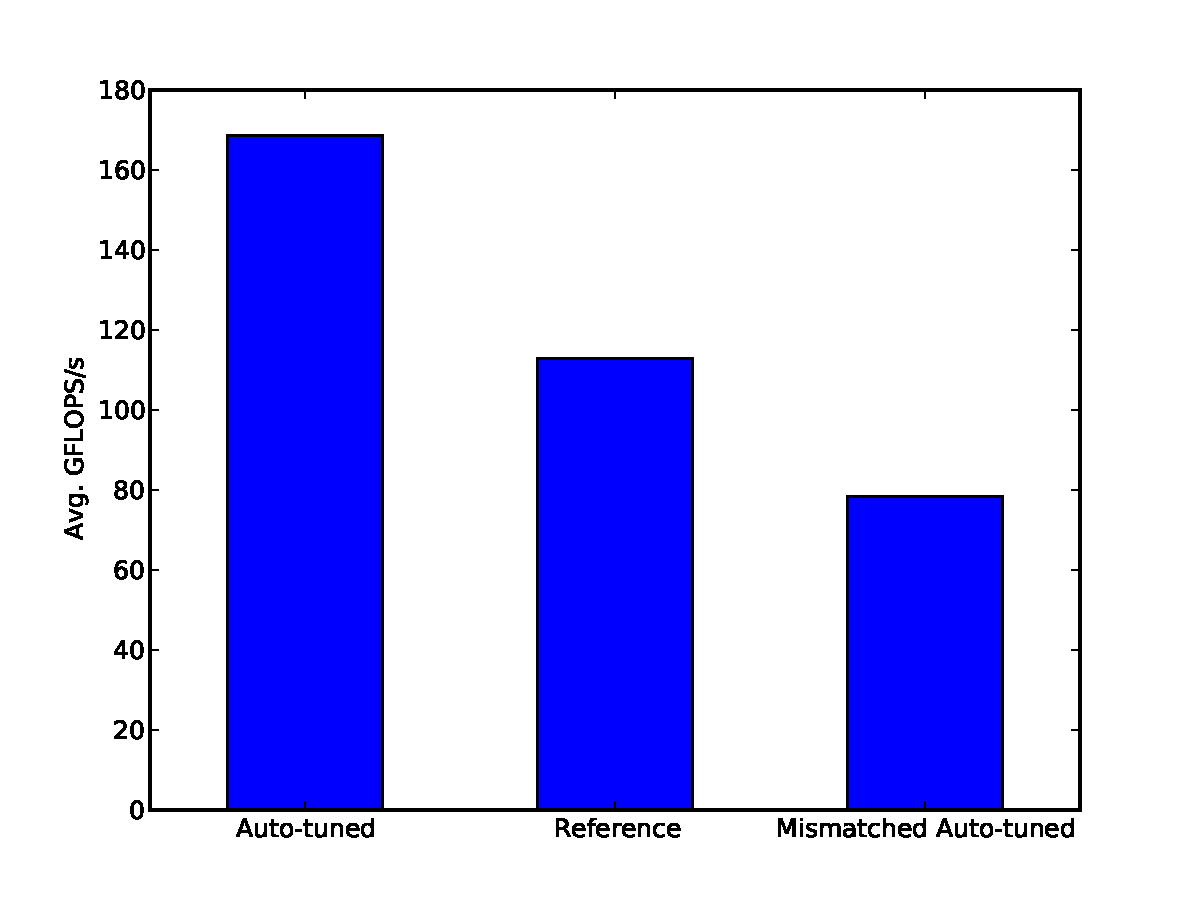
\includegraphics[scale=.42]{allstars_mixup_295.pdf}
\caption{Different arguments call for different kernels: each point corresponds to a randomly drawn argument configuration.
The reference speed (horizontal) is completely uncorrelated to the speed of an optimal kernel for an unrelated argument configuration (trials performed on GTX 295).
Out of 100 random confurations, 38 (not shown) could not even be run using a kernel that was auto-tuned for different arguments.
Good performance across a variety of inputs requires {\em input-dependent auto-tuning}.
}
\label{fig:speedup}
\end{figure}

\begin{figure}
\centering
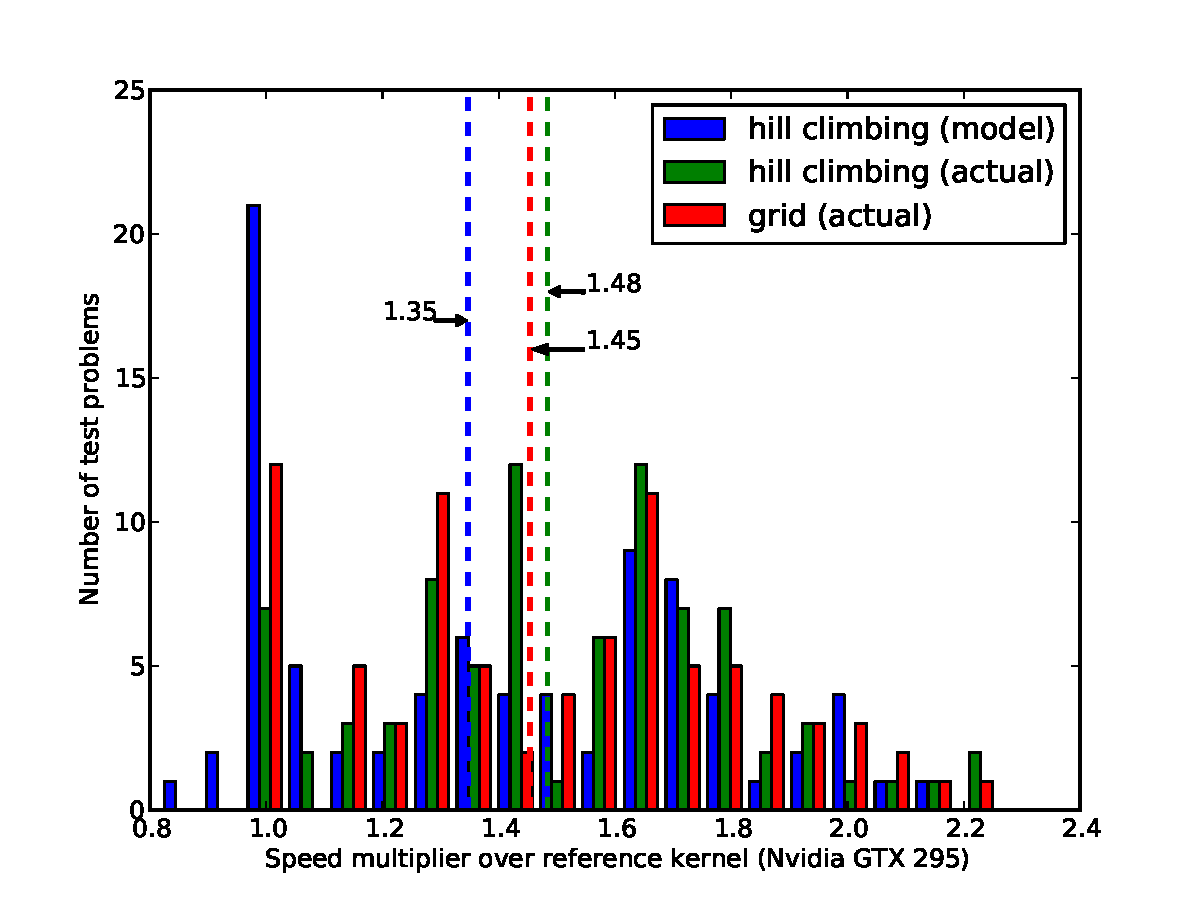
\includegraphics[scale=.42]{speedup_295.pdf}
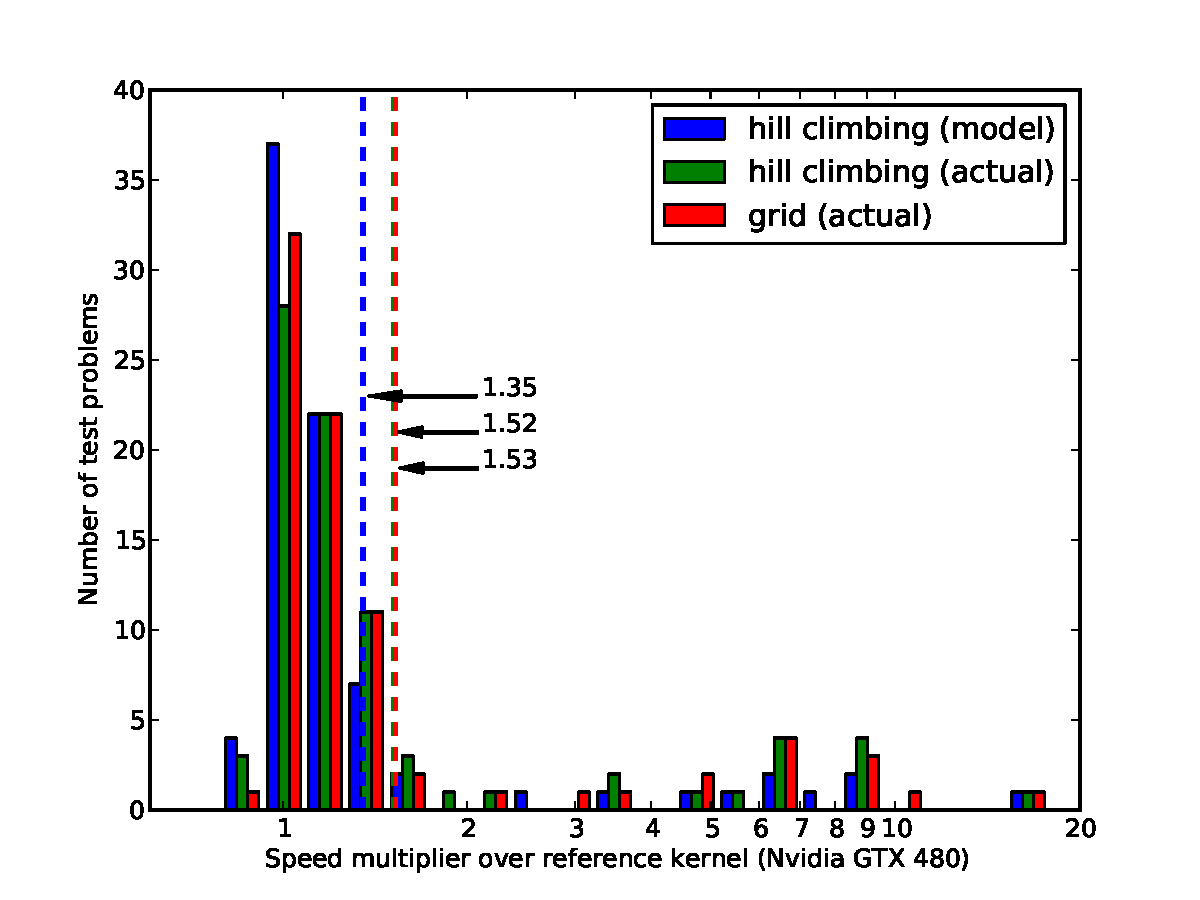
\includegraphics[scale=.42]{speedup_480.pdf}
\caption{Speedup of various auto-tuning strategies over the reference
implementation.
Each strategy was evaluated the same set of 83 problem configurations, which
was disjoint from the problem configurations used to build the model for
model-based hill-climbing.
The vertical dashed lines are positioned at the geometric mean speedup (XXX?)
of each strategy. The grid and hill-climbing approaches
tested 73 and 75 configurations respectively, and took 45?? XXX
seconds on average.
The model-based approach tested 0 configuration evaluations, and took 0.05
seconds on average, even with a naive Python implementation.
}
\label{fig:speedup}
\end{figure}


Figure~\ref{fig:speedup} also shows that random hill-climbing is at least
competitive and often better than the hand-chosen grid approach of ~\citet{pinto+cox:2011gcg}.  Figure~\ref{fig:hcX} shows how the number of hill-climbing iterations
affects the quality of the auto-tuned model.
The quicker HC25 approach is clearly inferior but the quality of the 75 iteration search (HC75) is statistically similar to the shorter HC50, suggesting that XXX.
Still, HC75 is not always better than the grid, so evidently neither search algorithm is perfect.

The previous figures establish that auto-tuning on a problem-by-problem basis can achieve good performance improvements over a high-quality reference baseline, but they do not show how long it takes to find these implementations.  A search of 75 iterations took an average of about 120 seconds XXX on a fast computer, because it requires compiling 75 CUDA kernels, and evaluating up to 750 filterbank correlations to get reliable timing information for each candidate implementation.

Our contrib

TL;DR: Hill-climbing is a good way to search the implementation space, can
search the full space and do about as well as grid search in the more
restricted space.


\begin{figure}
\centering
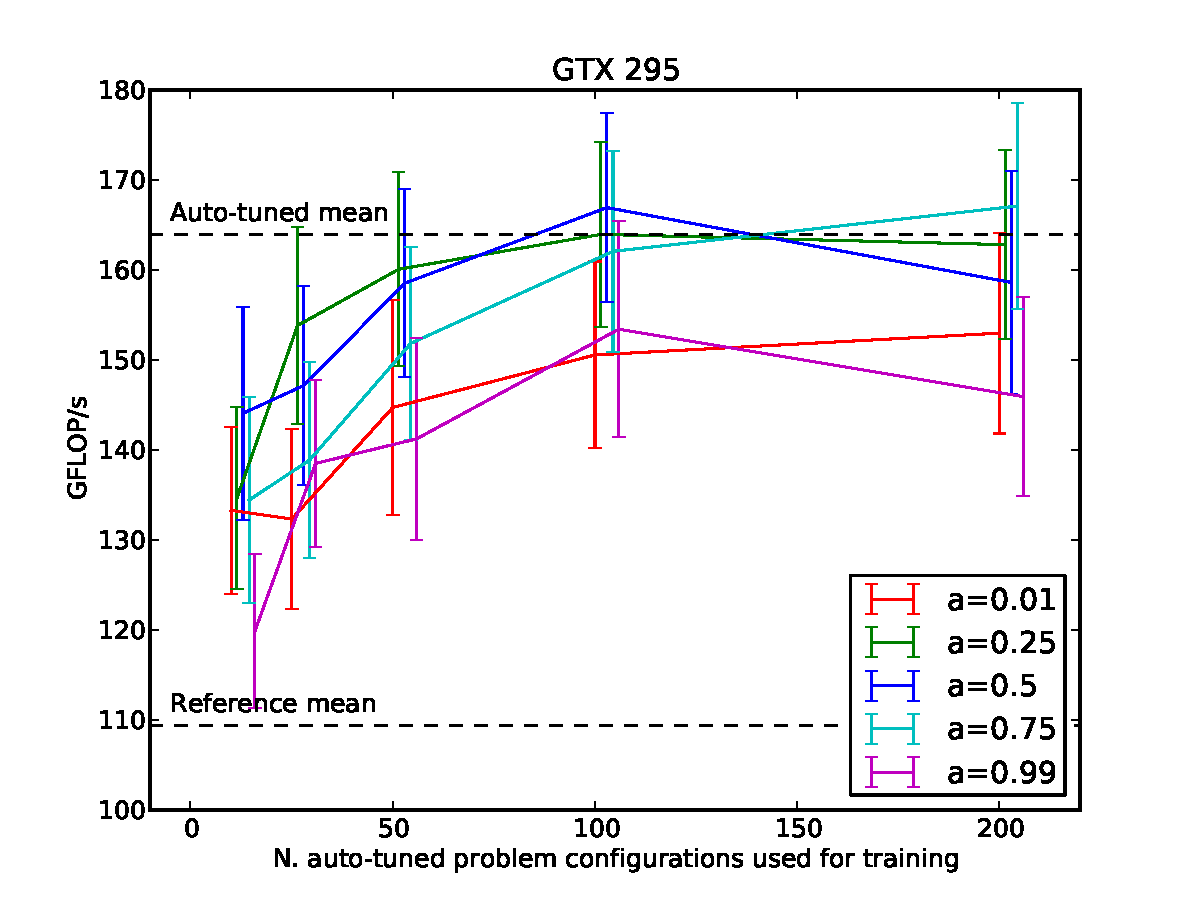
\includegraphics[scale=.42]{fig_ntrain_295.pdf} % on vader
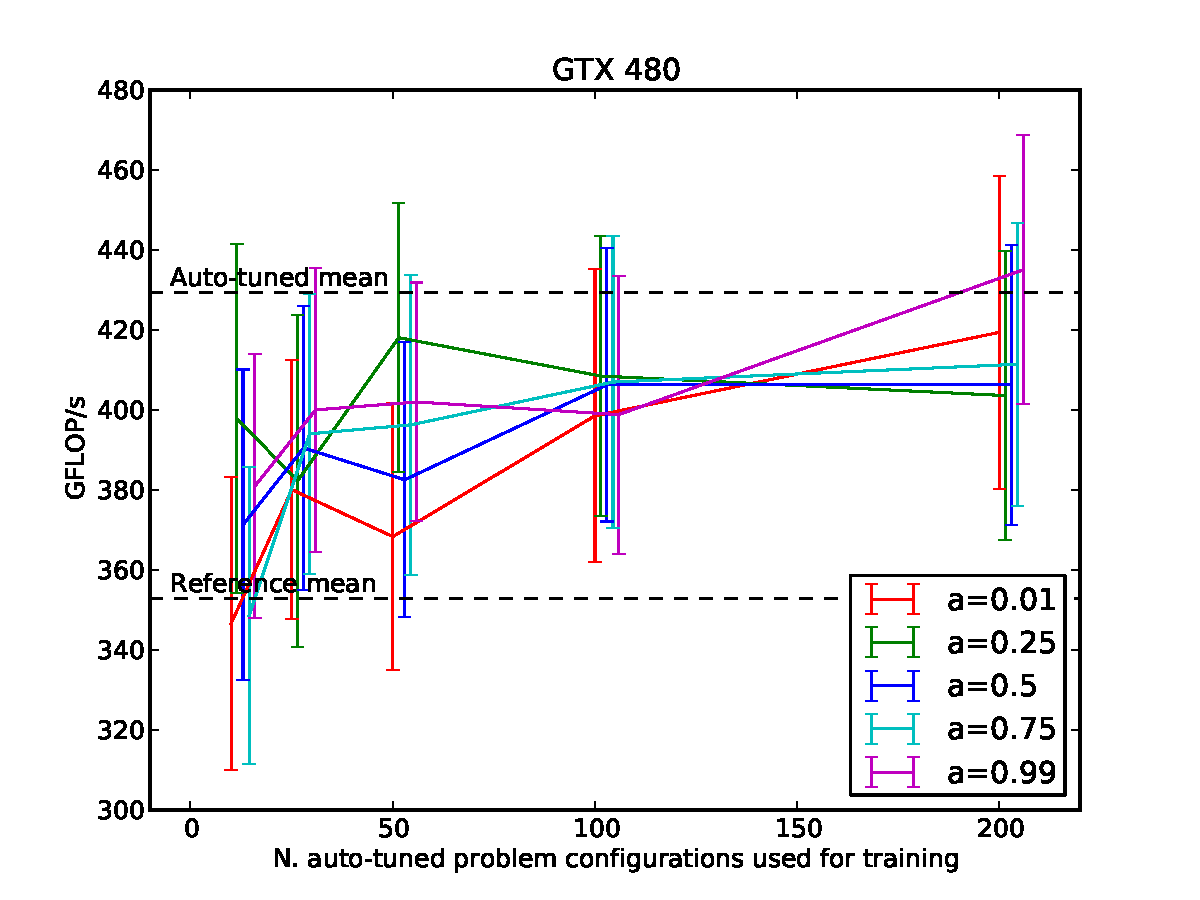
\includegraphics[scale=.42]{fig_ntrain_480.pdf} % on vader
\caption{The effect of the invalid configuration score ($a$) and training set
size on simulated auto-tuning.
All candidates timed during the grid and
hill-climbing search procedures were used as training points, so the training
set sizes ranged from an average of 1500 (10 problem configurations) to 30
thousand (200 problem configurations).
Training on 10 or 25 configurations was useful (higher mean than the reference),
but not as useful as training on 50 or more configurations.
The results on the GTX 295 suggest that
moderate values of $a$ between $0.25$ and $0.75$ might be
best, but $a$ had no significant effect on the GTX 480.
}
\label{fig:fig_ntrain}
\end{figure}

\begin{figure}
\centering
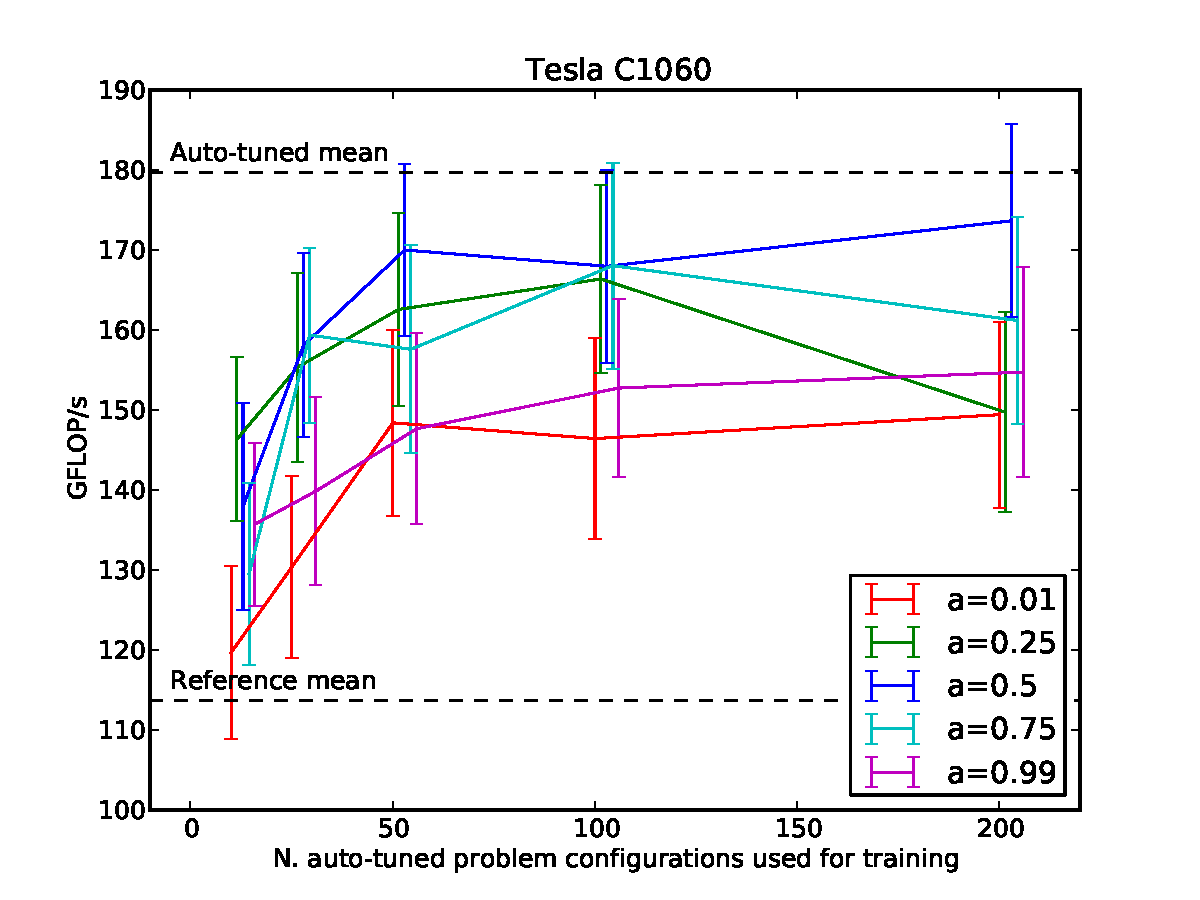
\includegraphics[scale=.42]{fig_ntrain_munctional0_1060.pdf}
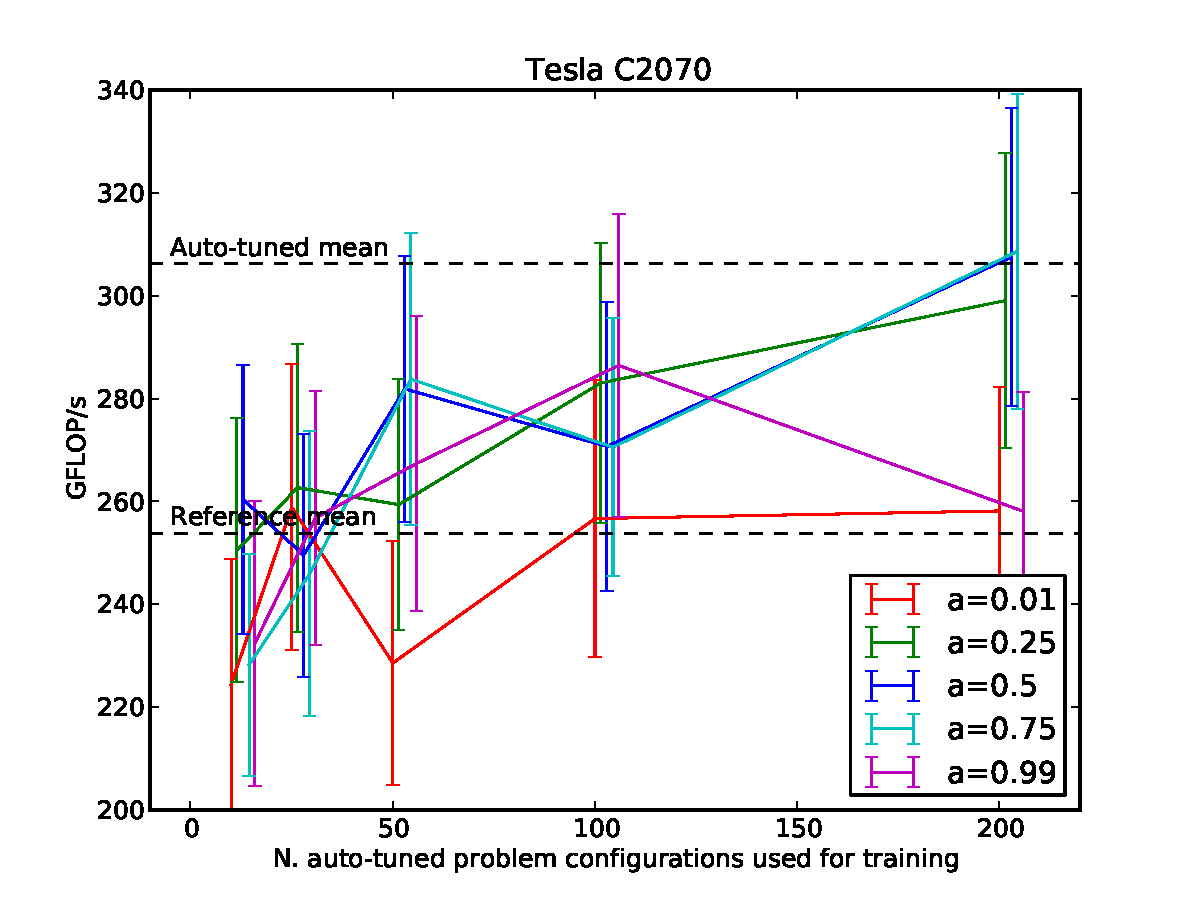
\includegraphics[scale=.42]{fig_ntrain_munctional0_2070.pdf}
\caption{more timing on munctional0}
\label{fig:fig_ntrain}
\end{figure}

\begin{figure}
\centering
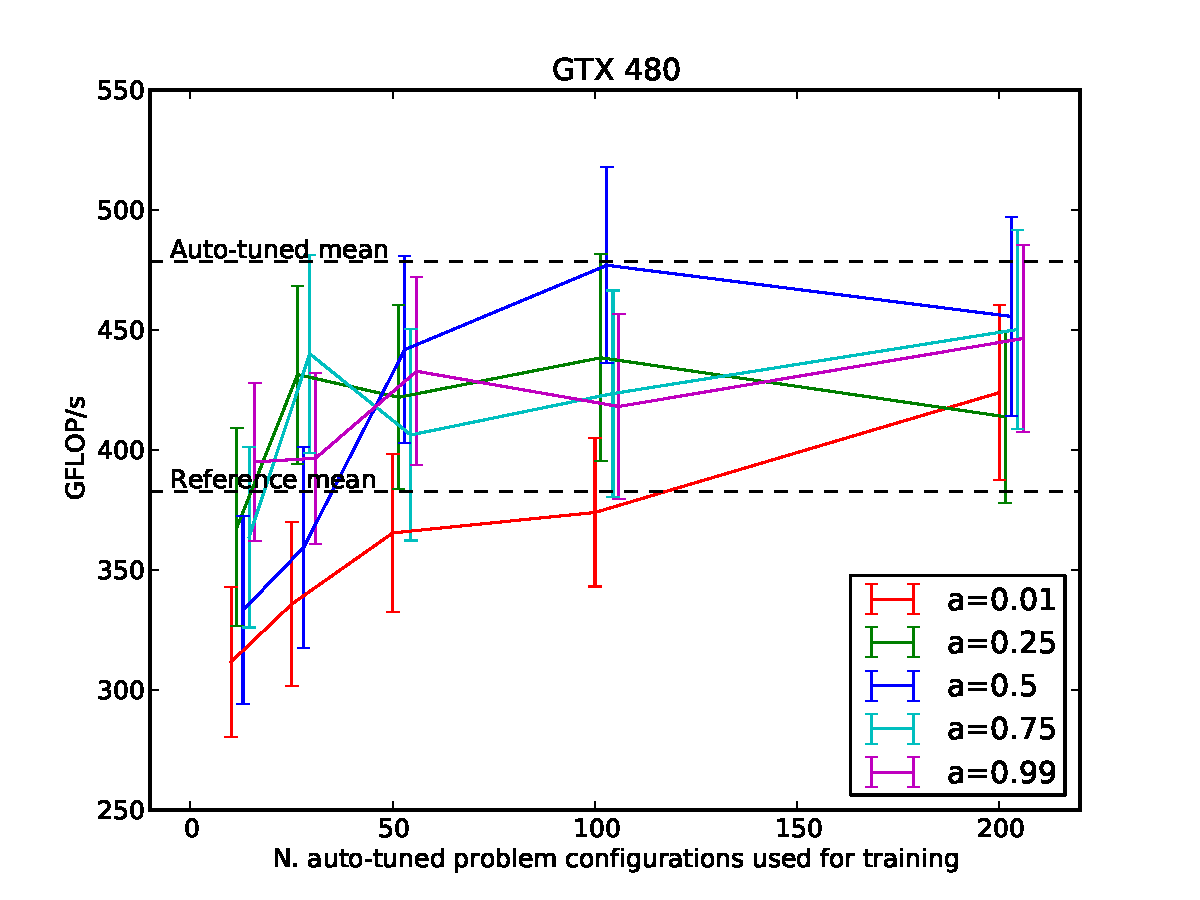
\includegraphics[scale=.42]{fig_ntrain_munctional0_480.pdf}
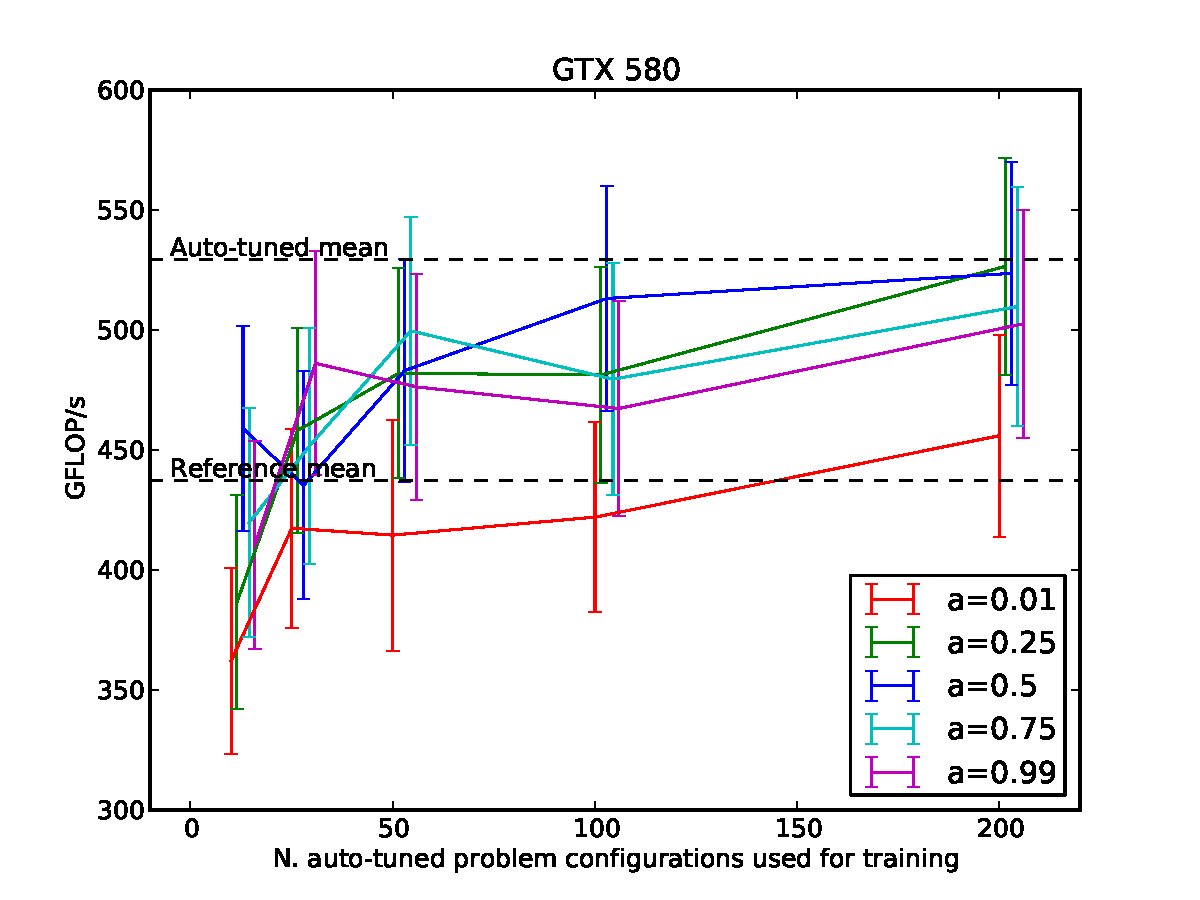
\includegraphics[scale=.42]{fig_ntrain_munctional0_580.pdf}
\caption{more timing on munctional0}
\label{fig:fig_ntrain}
\end{figure}

\begin{figure}
\centering
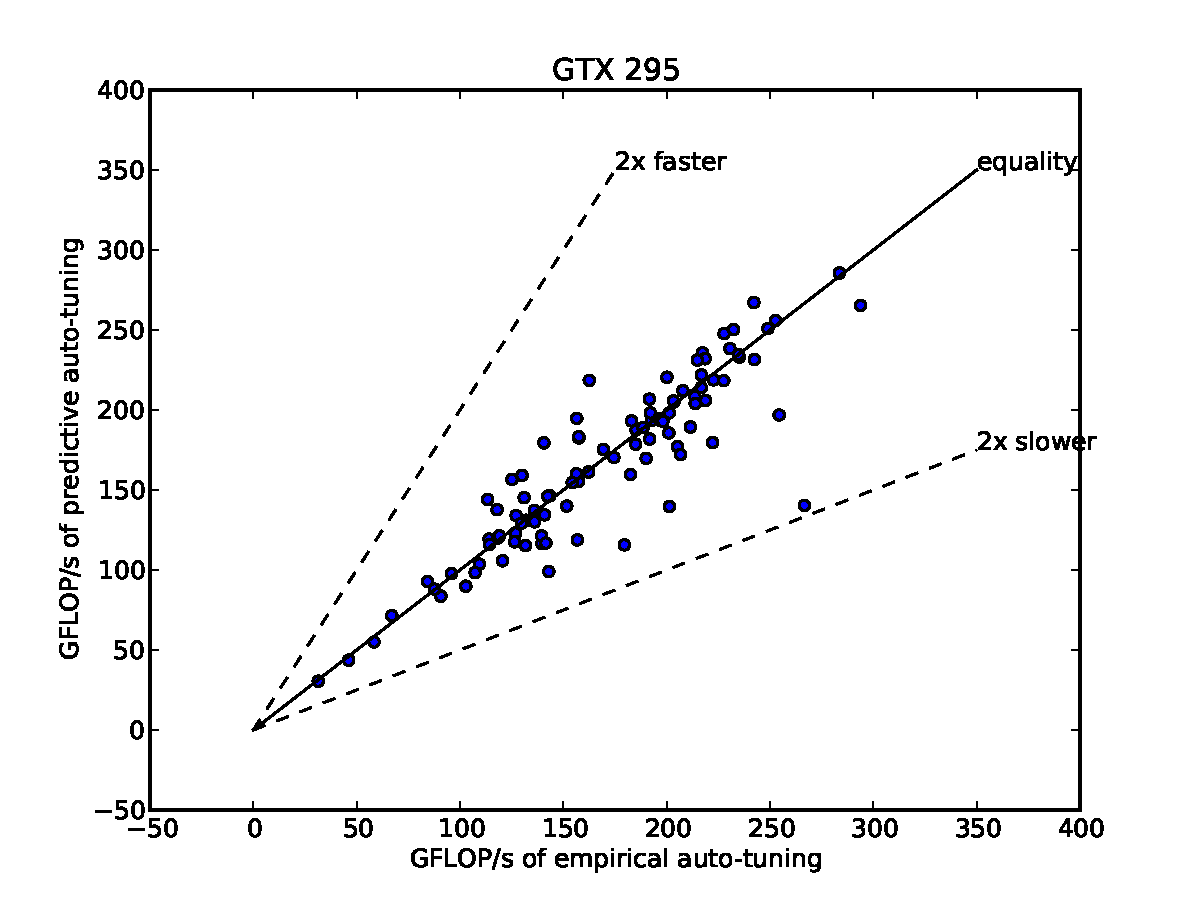
\includegraphics[scale=.42]{fig_gflop_scatter_295.pdf}
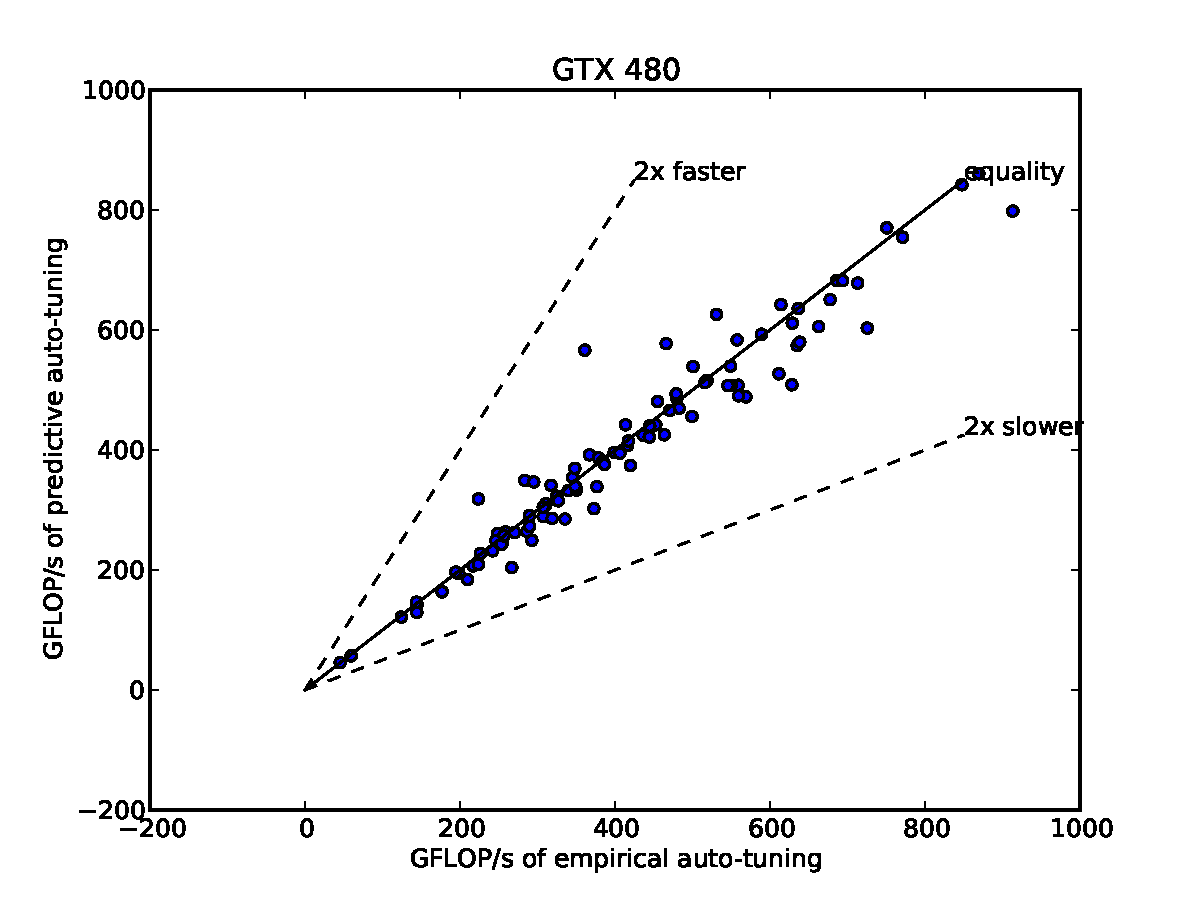
\includegraphics[scale=.42]{fig_gflop_scatter_480.pdf}
\caption{Computation speed for novel problem configurations using predictive
vs. empirical code specialization.
The scatterplots are roughly symmetric about the axis of equality (main diagonal)
with occasional outliers, indicating that for most problem configurations the
predictive approach gives as good a solution as the empirical approach.
The predictive approach typically requires about 0.1 seconds to suggest an
implementation, whereas the empirical approach requires about 2 minutes.
}
\label{fig:fig_gflop_scatter}
\end{figure}

\begin{figure}
\centering
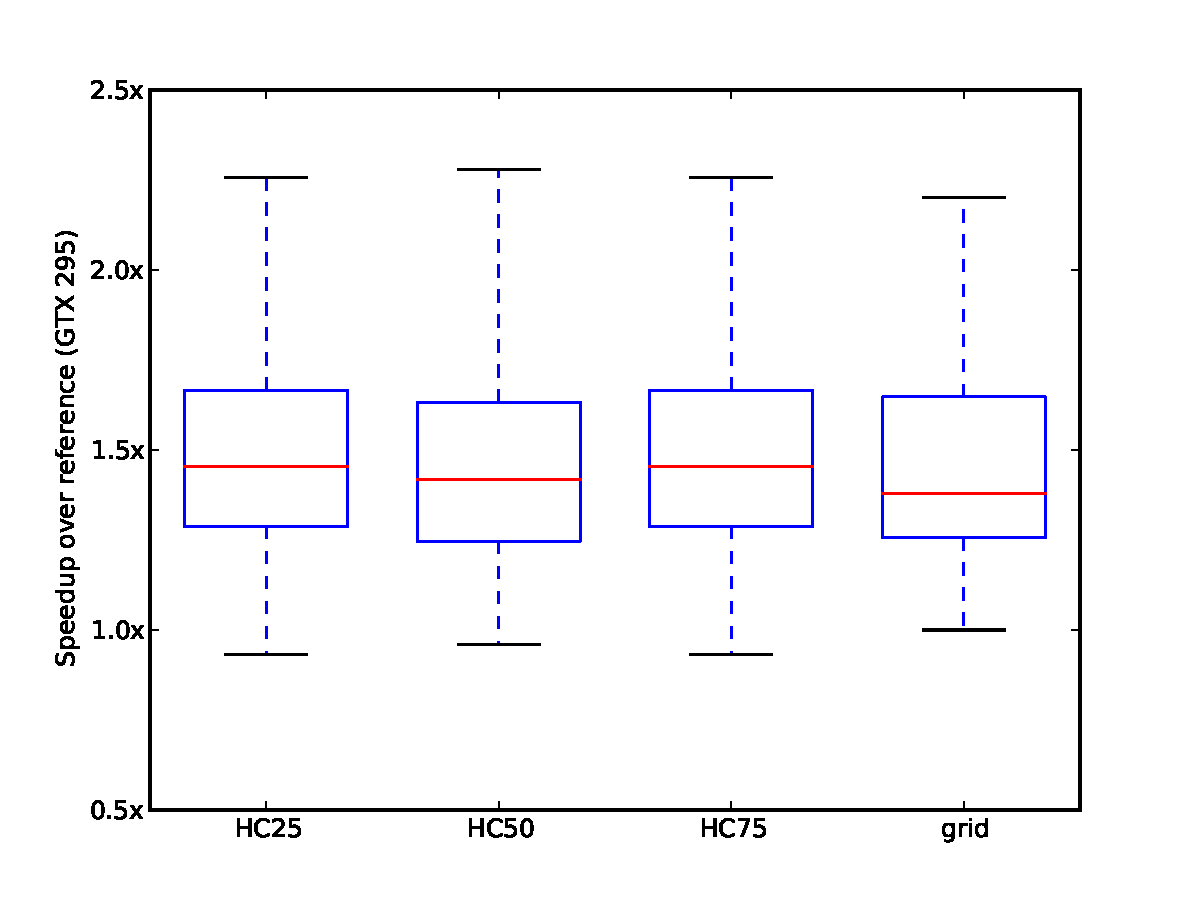
\includegraphics[scale=.42]{fig_genX_vader_295.pdf}
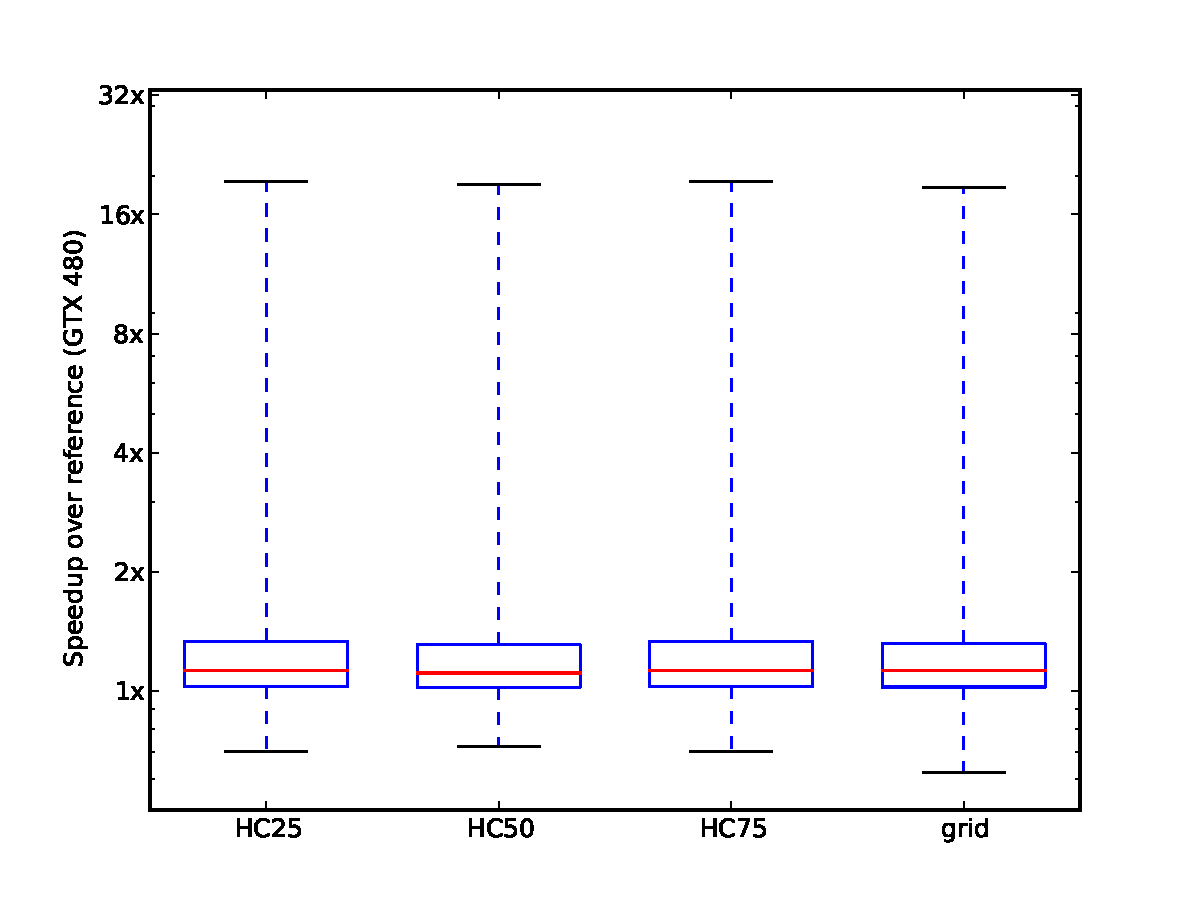
\includegraphics[scale=.42]{fig_genX_munctional0_480.pdf}
\caption{The speedup of hill-climbing (HC) and grid algorithms for empirical autotuning}
\label{fig:speedup}
\end{figure}

\begin{figure}
\centering
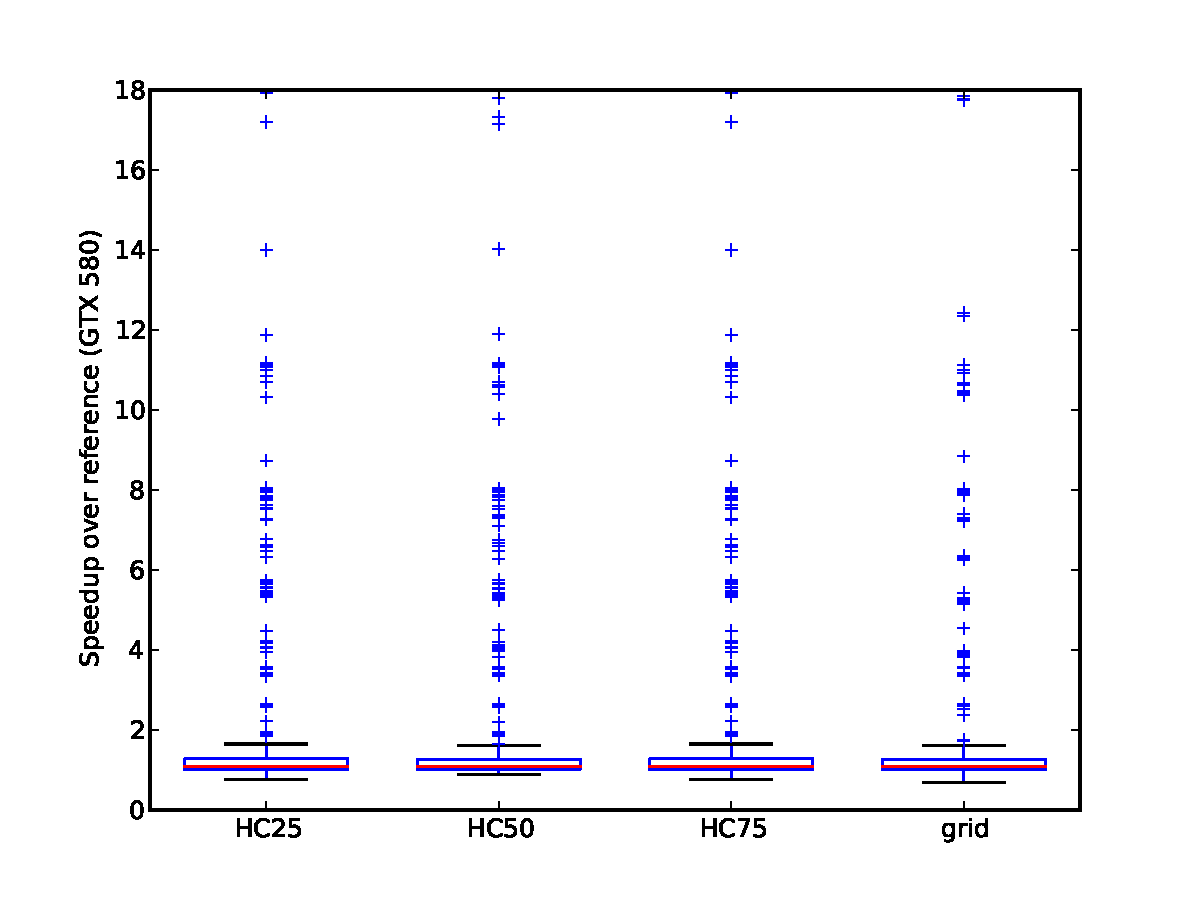
\includegraphics[scale=.42]{fig_genX_munctional0_580.pdf}
\caption{The speedup of hill-climbing (HC) and grid algorithms for empirical autotuning}
\label{fig:speedup}
\end{figure}

\begin{figure}
\centering
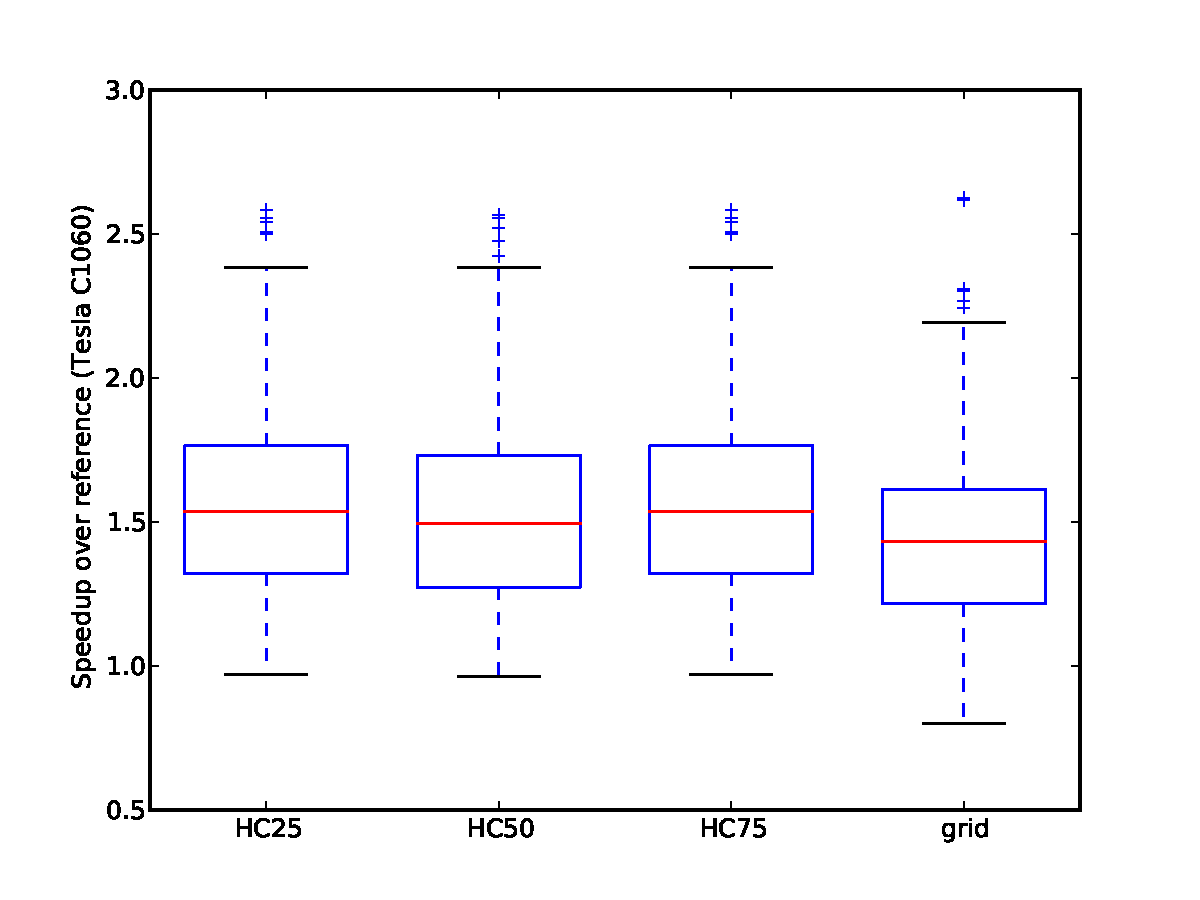
\includegraphics[scale=.42]{fig_genX_munctional0_1060.pdf}
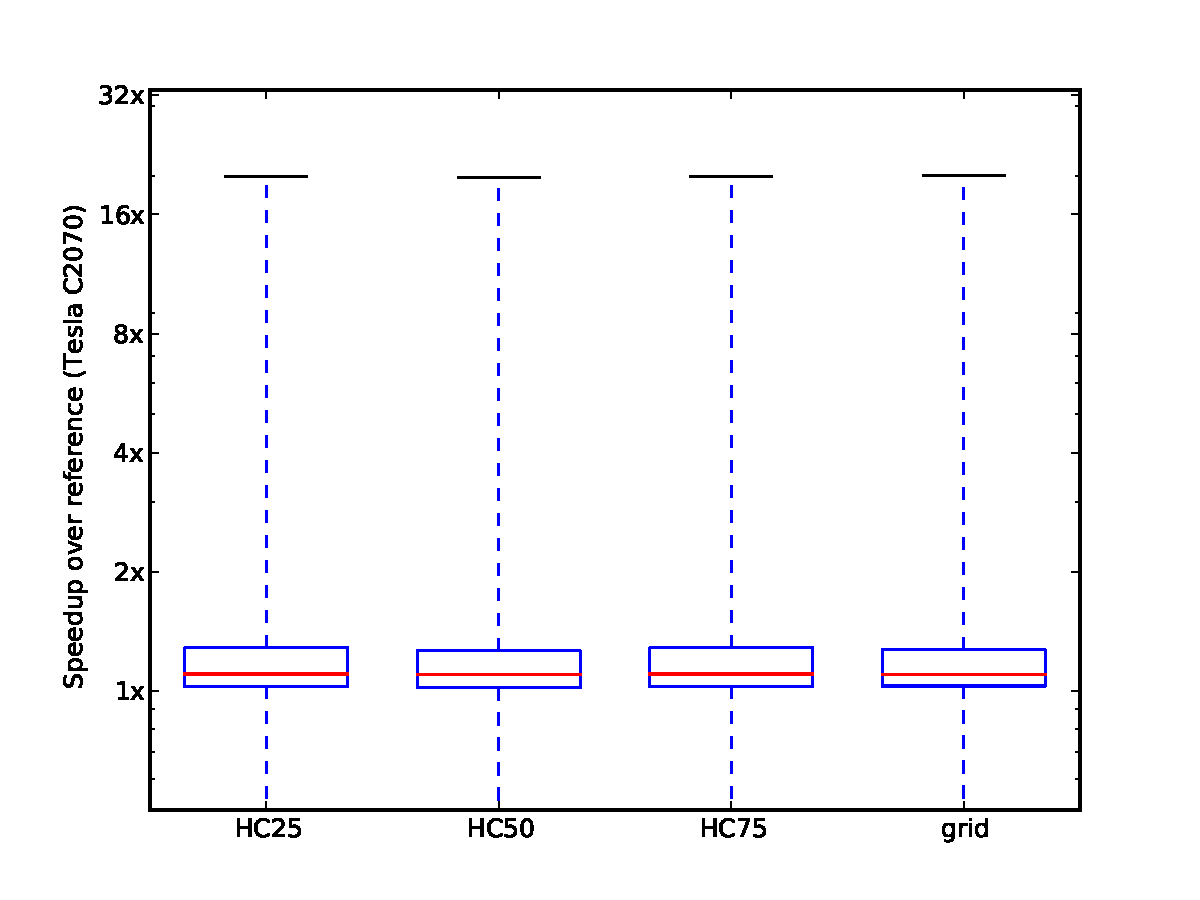
\includegraphics[scale=.42]{fig_genX_munctional0_2070.pdf}
\caption{The speedup of hill-climbing (HC) and grid algorithms for empirical autotuning}
\label{fig:speedup}
\end{figure}

\subsection{Model-based Autotuning}

On the GTX 295, a single regression-tree fit to the log-speed-multiplier
(LSM) function (XXX: how many problem configurations, how much vs. what
kind of training data) achieves an average Spearman correlation of 0.9 on
held-out test data (XXX: what kind of test data).

Now: the big test is that if we use the genetic search on the model instead of
the original function, do we get good performance?

\section{Discussion}

We're characterizing hardware by a 1-of-N feature vector, simply describing
which hardware is the current hardware.
To make better use of auto-tuning data from other platforms, it would be more
useful to have precise and descriptive features such as: what compute
capability is present, how many cores are active, what is the bandwidth
between the various kinds of memory, and how much of various kinds of memory
is present.  With these features a model-assisted auto-tuning approach
might be able to make very good guesses on hardware for which no auto-tuning
has ever been done.

In a complete implementation of Eq.~\ref{eq:z}, there would be parameters
related to the physical layout (e.g. strides) of $x$, $f$ and $z$ arrays in
addition to the mathematical parameters of heights and widths and so on,
so the total number of filterbank correlation computations that a user might
be able to demand is astronomical.
A typical coping mechanism would be to cast an arbitrary problem configuration into a more
standardized form, such as by copying inputs into aligned memory buffers with
appropriate padding, and then choosing an appropriate blocking strategy for
the computation. At that point, auto-tuning efforts can be focussed on the
kernel for each blocked strategy. However, on GPU hardware, the cost of
aligning the inputs can be relatively large.  In future work we hope to apply
our model-based technique to auto-tune in full problem configuration space, so
that we can optimize as much of the computation as possible within the
predictive auto-tuning framework (XXX name).

Platform Space: XXX

XXX: GCG chapter pg 13 notes that among the grid search, the best parameter
setting is different for the various platforms.

XXX: so far we only tried 3 cards... so we're using a 1-of-N feature.


%\renewcommand{\bibsection}{\section*{Bibliography}}
%\setlength{\bibsep}{5pt}
\bibliography{local}
\end{document}



One might expect then, that it would be easy to implement a library providing
this operation -- this hypothetical library could have quite a simple interface
following the spirit of FFTW or a BLAS routine:
\begin{verbatim}
    gpu_fbcorr(
        img_shape, filters_shape,
        img, filters, output)
\end{verbatim}
However, as shown in \citet{pinto+cox:2011gcg} and numerous articles on
related stencil operations XXX, it is challenging to provide an implementation
or even an implementation strategy that provides satisfactory performance
across the range of inputs (shapes, physical layouts) that occur even in
typical usage.

Current state-of-the art is to do empirical auto-tuning.
XXX \vspace{12pt}

Increasingly, machine learning and statistical inference strategies are
finding application in compiler technology.
XXX \vspace{12pt}

machine learning

This paper shows that a kernel with several  boosted


There is a natural function from
problem space x implementation space x platform space to runtime:
how much wall time elapses on the given platform when solving the given
problem with the given implementation.

Auto-tuning is a family of empirical techniques for finding the implementation
that minimizes that runtime function, when the platform and the problem
configuration are given.

XXX: some math, or possibly a picture with the three boxes that was on Pinto's
whiteboard.

This paper is about different ways of doing the minimization.
For a particular problem (filterbank correlation) we
look at a parameterized kernel implementation (from GCG)
and a few hardware platforms, and compare
random search, grid search, and a hill-climbing strategy with a good, but
generic, reference implementation.
Then we show that we can model the LSM function with a regression tree
well enough to usefully perform the argmin of Equation~\ref{eq:lsm_argmin}
on the model rather than the actual system. Whereas it may take several
minutes to perform a hill-climbing or grid search in the original system,
a hill-climbing search in the model requires a small fraction of a second.
Model-based autotuning makes it possible to simulate auto-tuning quickly and
accurately enough to be used within a single library call of the computational
routine.

Best arithmetic density

A bandwidth analysis that takes the blocking structure into account would
reveal that larger $H$ and $W$ require each block to read a larger input
region, and store it in a larger shared memory region, which reduces the
potential for high occupancy.

Filterbank correlation represents a difficult code-optimization problem
because of the number of interacting constraints: a large value of $P$ reduces
arithmetic density, but a small value of $P$ requires that each thread do more
work, and makes global memory access latency harder to hide. (XXX: is there a
better reason?)


The kernel used to perform
filterbank correlation was parametrized by 10 parameters, some of which
were binary and others of which were integer-valued. The full configuration
space included 12000 kernels.
XXX: how to make sense of these paramters without code listing?

XXX: What to all the parameters mean?
XXX: Point to github / GCG for full code listing.

XXX: how many configurations are in the configuration space

XXX: what was the reference kernel, and how was it chosen?

XXX: analysis of READ traffic, WRITE traffic, DATA re-use and CACHEing
strategies. FLOPS per write etc.

XXX: Why not use FFT: convolution in spectral domain?

XXXX: Talk about memory transfer requirements vs. speed vs. copy...


